\chapter{Proposed Methodology}
\label{ch:methodology}

\section{Overview}

\textbf{Goal.} ChromaGuide is a three-component framework for \sgRNA\ design that couples (i) \textbf{on-target efficacy prediction}, (ii) \textbf{off-target prediction} (unintended cleavage-site risk), and (iii) an \textbf{integrated \sgRNA\ design score} that balances predicted efficiency and specificity.

\textbf{Task 1 (on-target).} Given a guide/target pair in a cellular context, predict on-target efficacy $y\in[0,1]$ and (optionally) output a prediction interval with target coverage $1-\alpha$.

\textbf{Task 2 (off-target).} Given a candidate \sgRNA\ and a reference genome, identify plausible unintended cleavage sites and score their cleavage likelihood/severity, producing an aggregated off-target risk summary.

\textbf{Task 3 (design score).} Combine the calibrated on-target signal with the aggregated off-target risk to produce an overall \sgRNA\ design score for ranking candidate guides.

\textbf{Inputs.}
\begin{itemize}
\item \textbf{Sequence} $x_s$: \sgRNA\ protospacer+\PAM{} and target-site sequence context.
\item \textbf{Epigenomics} $x_e$: accessibility/histone-mark tracks summarized in a fixed window around (on-target and, when available, off-target) cut sites.
\item \textbf{Genome index/search} $\mathcal{G}$: reference genome data structure used to enumerate candidate off-target loci.
\end{itemize}

\textbf{Core modules (baseline design; alternatives are evaluated via ablation).}
\begin{itemize}
\item On-target encoders: sequence encoder $z_s=g_s(x_s)$ and epigenomic encoder $z_e=g_e(x_e)$.
\item On-target fusion: $z=f([z_s;z_e])$ (baseline concatenation; optional attention/gating; optional non-redundancy regularizer).
\item On-target head: bounded-outcome head producing $(\mu,\phi)$ (baseline Beta regression) and conformal prediction for calibrated intervals~\citep{vovk2005,romano2019,barber2023}.
\item Off-target candidate generation: enumerate candidate loci using genome-wide approximate matching (PAM-constrained) with a bounded mismatch/bulge policy.
\item Off-target scoring network: score each candidate off-target site using sequence mismatch features and optional local context features (sequence, chromatin accessibility when available).
\item Design-score aggregator: combine the on-target prediction with an aggregated off-target risk to produce a single \sgRNA\ design score.
\end{itemize}


\begin{figure}[htbp]
\centering
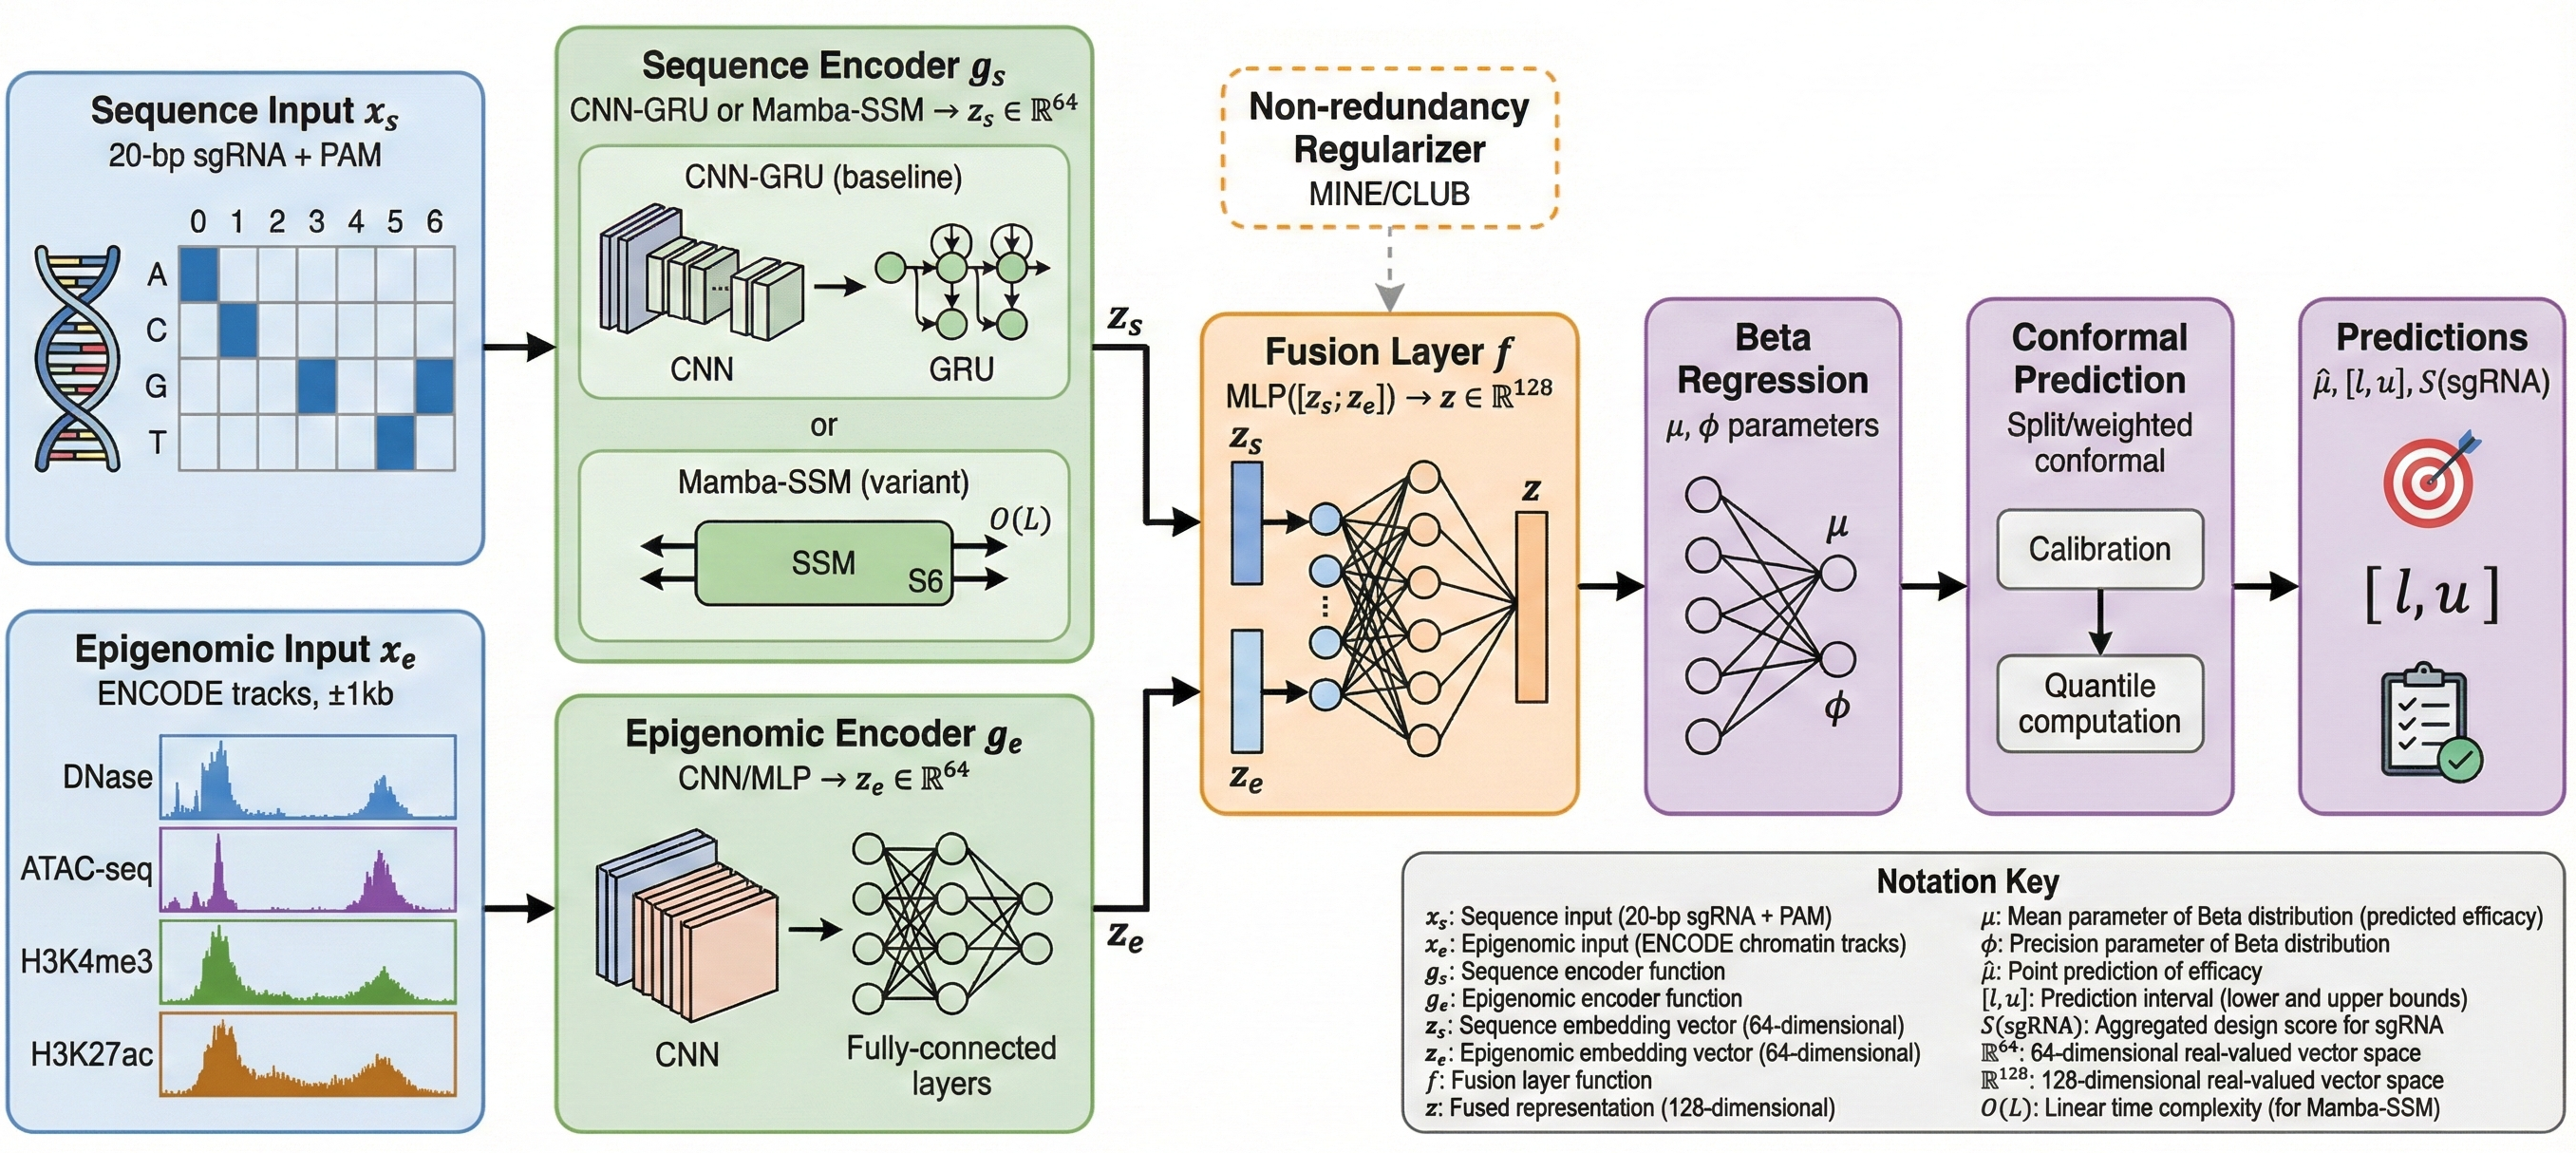
\includegraphics[width=\textwidth]{Figs/ChromaGuide.png}
\caption{ChromaGuide architecture overview. The framework fuses sequence representations with epigenomic context features through a fusion layer. The sequence encoder supports two architectures: (1) a CNN-GRU baseline, or (2) a Mamba-based state-space model (SSM) variant with bi-directional processing and $O(L)$ linear complexity. Inputs: $\mathbf{x}_s$ (one-hot encoded 23-nt sgRNA+PAM sequence (20-nt protospacer + 3-nt PAM)), $\mathbf{x}_e$ (epigenomic tracks). Encoders: $g_s$ (sequence encoder) and $g_e$ (epigenomic encoder) produce embeddings $\mathbf{z}_s, \mathbf{z}_e \in \mathbb{R}^{64}$. Fusion layer $f$ produces $\mathbf{z} \in \mathbb{R}^{128}$. Beta regression outputs parameters $\mu$ (mean) and $\phi$ (precision). Conformal prediction generates calibrated intervals. Final outputs: point prediction $\hat{\mu}$, prediction interval $[l, u]$, and design score $S(\text{sgRNA})$. Optional non-redundancy regularizer (MINE/CLUB) encourages complementary representations.}
\label{fig:proposed-architecture}
\end{figure}

\section{Model architecture}


\subsection{\texorpdfstring{Sequence encoder $g_s$}{Sequence encoder gs}}

\begin{sloppypar}
Baseline: ChromeCRISPR-style CNN--GRU on 23-nt sgRNA+\PAM{} (CNN kernels 3/5/7 $\to$ BiGRU hidden 128 $\to$ pooled $z_s\in\mathbb{R}^{64}$). As contemporary alternatives, we will evaluate (i) hybrid architectures with dynamic feature weighting as in CRISPR\_HNN~\citep{li2025crisprhnn} and (ii) pretrained language-model embeddings for cross-variant generalization as in PLM-CRISPR~\citep{hou2025plmcrispr}. Transformer-based DNA/RNA embeddings (e.g., DNABERT-2, Nucleotide Transformer) and state-space model (SSM) backbones (e.g., Mamba) are included as planned architectural ablations to determine whether modern pretrained representations improve upon the CNN-GRU baseline inherited from ChromeCRISPR.
\end{sloppypar}

\textbf{Structured ablation protocol.} Table~\ref{tab:ablation-backbone} specifies the backbone comparison design. All ablations share identical downstream components (same fusion layer, same prediction head, same training budget of 100 epochs on a single A100 GPU), varying only the sequence encoder. Selection criteria: the backbone yielding the highest validation Spearman $\rho$ on Split~A (gene-held-out) is adopted as the final encoder; ties are broken by parameter count (fewer preferred).

\begin{table}[h]
\centering
\small
\caption{Structured backbone ablation design. All conditions use identical fusion, head, and training configuration.}
\label{tab:ablation-backbone}
\begin{tabular}{llccc}
\hline
\textbf{Backbone} & \textbf{Type} & \textbf{Params (M)} & \textbf{Pretrained} & \textbf{$d_{\text{out}}$} \\
\hline
CNN-GRU (baseline) & Convolutional+Recurrent & $\sim$2 & No & 64 \\
DNABERT-2 & Transformer (6-mer) & $\sim$117 & Yes & 64 \\
Nucleotide Transformer & Transformer (6-mer) & $\sim$500 & Yes & 64 \\
Caduceus-PS & Mamba SSM (bi-dir) & $\sim$7 & Yes & 64 \\
Evo (7B, frozen+adapter) & StripedHyena & $\sim$14 (adapter) & Yes & 64 \\
\hline
\end{tabular}
\end{table}

\begin{sloppypar}
Beyond Transformers, we will explore \textbf{state-space models (SSMs)} as an alternative sequence encoder architecture. Mamba~\cite{gu2023mamba} introduced selective state spaces with input-dependent gating, achieving linear-time complexity $O(L)$ while maintaining expressive long-range modeling. For genomic applications, Caduceus~\cite{schiff2024caduceus} extended Mamba with bi-directional processing and reverse-complement (RC) equivariance, demonstrating superior performance on long-range DNA sequence tasks at the ICML 2024 conference. The Evo model~\cite{nguyen2024evo} scaled long-context genome modeling to 131kb using the StripedHyena architecture (a hybrid attention + long convolution design), demonstrating that long-range encoders can capture regulatory elements across large genomic loci. Recent work has shown that pre-trained DNA language models can substantially improve CRISPR on-target efficacy prediction when fine-tuned on guide-specific datasets~\citep{li2025crisprfmc,hou2025plmcrispr}, motivating the use of foundation model encoders in our sequence branch. Separately, DNABERT-Epi~\citep{kimata2025dnabertepi} demonstrated that integrating epigenetic features with pre-trained DNA language models significantly improves CRISPR \emph{off-target} prediction; we leverage a similar epigenomic integration strategy in our off-target module (Section~\ref{sec:offtarget}). We will benchmark a Mamba-based variant of our sequence encoder against the CNN-GRU baseline, evaluating whether SSMs provide computational efficiency gains without sacrificing predictive accuracy for sgRNA design tasks.
\end{sloppypar}


\subsection{\texorpdfstring{Epigenomic encoder $g_e$}{Epigenomic encoder ge}}

For each assay (e.g., DNase/ATAC, H3K4me3, H3K27ac), extract a window (default $\pm 1$ kb) around the cut site, bin into fixed-length features, apply log1p and training-only standardization, and map through an MLP to $z_e\in\mathbb{R}^{64}$. Additional tracks/encoders (e.g., 1D CNNs over binned tracks) are evaluated in ablation as alternative architectures for epigenomic encoding if the baseline MLP proves insufficient. 

\textbf{ENCODE cell-line mapping.} The DeepHF benchmark uses three cell lines: HEK293T, HCT116, and HeLa. We source matched epigenomic tracks from the ENCODE portal~\citep{encode2020} as follows: (i)~\textbf{HEK293T}: DNase-seq (ENCSR000ENM), H3K4me3 ChIP-seq (ENCSR000DTU), and H3K27ac ChIP-seq (ENCSR000FCJ); (ii)~\textbf{HCT116}: DNase-seq (ENCSR000ENO), H3K4me3 ChIP-seq (ENCSR000DWN), and ATAC-seq (ENCSR000EOJ); (iii)~\textbf{HeLa}: DNase-seq (ENCSR000ENP), H3K4me3 ChIP-seq (ENCSR000DWE), and H3K27ac ChIP-seq (ENCSR000FCG). All signal tracks are aligned to hg38 and processed as fold-change-over-control bigWig files. For cell lines where a specific assay is unavailable, we set the corresponding input channel to zero and include an assay-availability indicator feature. This explicit mapping ensures that ChromaGuide's multi-modal premise is grounded in concrete, reproducible, and empirically justified data sources. These three tracks were selected because they capture complementary aspects of the chromatin environment relevant to \CasNine\ access: DNase-seq/ATAC-seq directly measures physical DNA accessibility at the cut site, H3K4me3 marks active promoter regions where guide targeting is most frequent, and H3K27ac identifies active enhancers and regulatory elements where chromatin state modulates cleavage efficiency. Together they provide broad coverage of ENCODE-profiled cell types while remaining tractable for multi-modal training; repressive marks (e.g., H3K9me3, H3K27me3) are excluded from the default set but may be explored in ablation studies.

\subsection{\texorpdfstring{Fusion $f$ and optional non-redundancy regularizer}{Fusion f and optional non-redundancy regularizer}}

Our proposed default fusion strategy is \textbf{gated attention fusion}, selected based on preliminary experiments; the final choice will be determined by systematic ablation comparison and may be revised if alternative strategies (e.g., cross-attention or mixture-of-experts) demonstrate superior performance: $z=\mathrm{GatedAttn}([z_s;z_e])\in\mathbb{R}^{128}$, where a learned gating vector $g=\sigma(W_g[z_s;z_e]+b_g)$ modulates the element-wise contribution of each modality before a final projection layer. This mechanism was selected because (i) it allows the model to dynamically weight sequence vs.\ epigenomic features per sample, which is critical when chromatin accessibility varies across cell lines, and (ii) gated fusion has demonstrated superior performance over simple concatenation in related multi-modal genomics tasks. As planned ablations, we additionally evaluate concatenation+MLP, cross-attention, and mixture-of-experts fusion to validate this design choice (see Table~\ref{tab:ablation-backbone}). Hyperparameter optimization will be conducted via \textbf{Bayesian optimization} using the Optuna framework~\citep{akiba2019optuna} with a Tree-structured Parzen Estimator (TPE) sampler over 50 trials, optimizing validation Spearman $\rho$ on Split~A. The search space includes learning rate ($[10^{-5}, 10^{-2}]$ log-uniform), dropout rate ($[0.05, 0.4]$), hidden dimension ($\{64, 128, 256\}$), batch size ($\{32, 64, 128\}$), and fusion gate initialization bias ($[-1, 1]$). Early stopping with patience of 15 epochs prevents overfitting during each trial.

We optionally encourage complementary representations with an information-theoretic objective:
\begin{equation}\label{eq:fusion}
f^* = \arg\max_{f \in \mathcal{F}} \left[ I(f(X_s, X_e); Y) - \lambda \cdot I(X_s; X_e | Y) \right],
\end{equation}
implemented with neural MI estimators (e.g., MINE/CLUB)~\citep{belghazi2018,cheng2020} and treated strictly as an ablation.

\subsection{Prediction head (Beta regression)}

Predict a Beta mean and precision:
\begin{equation}
\mu = \sigma(W_\mu z + b_\mu),\qquad \phi = \exp(W_\phi z + b_\phi).
\end{equation}
Negative log-likelihood:
\begin{equation}\label{eq:beta_loss}
\begin{split}
L = -\sum_{i=1}^N \Big[ &\log \Gamma(\phi_i) - \log \Gamma(\mu_i \phi_i) - \log \Gamma((1-\mu_i)\phi_i) \\
&\quad + (\mu_i \phi_i - 1) \log y_i + ((1-\mu_i)\phi_i - 1) \log(1-y_i) \Big].
\end{split}
\end{equation}
We clip $y$ to $(\varepsilon,1-\varepsilon)$ when needed; Beta regression is standard for continuous outcomes in $(0,1)$~\citep{ferrari2004beta}.

\section{Uncertainty quantification via conformal prediction}

Split conformal prediction yields distribution-free prediction intervals \emph{under the exchangeability assumption}~\citep{vovk2005,romano2019}. With a Beta head, define
$$
\hat{\sigma}=\sqrt{\frac{\hat{\mu}(1-\hat{\mu})}{1+\hat{\phi}}},\qquad s=\frac{|y-\hat{\mu}|}{\hat{\sigma}+\varepsilon}.
$$
On calibration data compute $\hat{\eta}=\mathrm{Quantile}_{1-\alpha}(\{s_i\})$ and output
$$
C(x)=\left[\hat{\mu}(x)-\hat{\eta}\,\hat{\sigma}(x),\;\hat{\mu}(x)+\hat{\eta}\,\hat{\sigma}(x)\right]\cap[0,1].
$$
For dataset/cell-line shift (Splits B/C), use weighted conformal calibration, which relies on (estimated) importance weights / likelihood ratios and may degrade under severe shift~\citep{barber2023}.

\section{Off-target prediction  module}

\textbf{Exchangeability under gene-held-out evaluation.} For Split~A (gene-held-out), we acknowledge that strict exchangeability may not hold because guides targeting different genes inhabit distinct genomic contexts with varying GC content and chromatin environments. We address this through two complementary strategies. First, we empirically verify approximate exchangeability by comparing the marginal feature distributions (sequence composition, predicted secondary structure energy, and epigenomic signal statistics) between calibration and test gene groups using two-sample Kolmogorov--Smirnov tests; if the null hypothesis of identical distributions is not rejected at $\alpha=0.05$ for all features, we report standard conformal coverage. Second, as a robustness check, we apply weighted conformal prediction to Split~A using gene-level importance weights estimated via logistic regression on a binary gene-group indicator, following the framework of \citet{barber2023}. We report both the standard and weighted coverage for Split~A, clearly distinguishing between the finite-sample guarantee (valid only under exchangeability) and the empirical coverage (always reported). If weighted and standard coverage diverge by more than 2 percentage points, we flag the gene-held-out split as exhibiting non-trivial covariate shift and interpret the conformal intervals as approximate rather than distribution-free. \textbf{Marginal vs.\ conditional coverage.} We note that standard conformal prediction provides \emph{marginal} coverage---i.e., averaged over all test points---rather than \emph{conditional} coverage for any specific input $x$. The gap between marginal and conditional coverage can be significant when the model's uncertainty varies across the input space (e.g., high-GC vs.\ low-GC guides, open vs.\ closed chromatin regions). To partially bridge this gap, we stratify the empirical coverage analysis by (i) GC-content quartile, (ii) chromatin accessibility quartile, and (iii) gene functional category, reporting per-stratum coverage alongside the global marginal rate. If per-stratum coverage falls below $(1-\alpha) - 0.05$ for any subgroup, we apply the group-conditional conformal procedure of~\citet{barber2023} to recalibrate intervals within that stratum, accepting the corresponding reduction in statistical efficiency.
\label{sec:offtarget}

\subsection{Candidate unintended-site identification}

Given a candidate \sgRNA{}, ChromaGuide first enumerates plausible off-target loci by scanning the reference genome for PAM-adjacent protospacer matches under an explicit mismatch/bulge policy. Concretely, we (i) require a valid PAM (e.g., NGG for SpCas9; optionally extend to alternative PAMs when modeling SpCas9 variants), (ii) allow up to $m$ mismatches with position-dependent weighting (penalizing mismatches less in distal regions than in the seed), and (iii) optionally allow a small number of DNA/RNA bulges, depending on computational feasibility.

This stage outputs a set of candidate off-target sites $\{o_j\}$, each with its genomic coordinates and an alignment summary (mismatch positions/types and bulge indicators). To keep the proposal implementable and the document within a $\sim$30-page scope, we treat the genome search as a modular component (e.g., using an indexed approximate matching routine) and focus the research contribution on learning to score the resulting candidate set.

\subsection{Off-target scoring}

For each candidate site $o_j$, we compute a feature vector that includes (a) aligned guide--DNA sequence pairs / mismatch pattern encodings, (b) local sequence context around the cut site, and (c) optional cell-context features (e.g., accessibility) when tracks are available for the corresponding locus. This is motivated by recent off-target models that integrate epigenetic tracks with sequence representations (e.g., DNABERT-Epi)~\citep{kimata2025dnabertepi}. A neural scoring function outputs a per-site risk $r_j\in[0,1]$ that is intended to correlate with cleavage likelihood and/or editing readouts in available off-target datasets.

\textbf{Training data.} The off-target scoring model is trained on experimentally validated off-target sites from GUIDE-seq~\citep{tsai2015guideseq} and CIRCLE-seq~\citep{tsai2017circleseq} datasets, which together provide $\sim$200k labeled guide--off-target pairs across multiple cell lines. Positive labels indicate biochemically or cellularly validated cleavage events; negatives are PAM-adjacent genomic sites with no detected cleavage above background. We apply the same gene-level deduplication strategy described in \S\ref{sec:evaluation} to avoid train/test overlap on homologous loci.

\textbf{Scoring architecture.} The per-site scoring function $f_{\text{OT}}$ is a three-layer convolutional neural network (CNN) with 1D convolutions over the aligned guide--target pair (kernel sizes 3, 5, 7 to capture local and extended mismatch context), followed by global average pooling and two fully connected layers ($d=128 \to 64 \to 1$) with a sigmoid output producing $r_j \in [0,1]$. When cell-specific chromatin features are available, they are concatenated after the pooling layer. The model is trained with binary cross-entropy loss and class-weight balancing to handle the strong negative-class imbalance ($\sim$50:1 in GUIDE-seq).

To summarize genome-wide risk for a guide, we aggregate across sites using a soft-max/Noisy-OR style pooling function, for example
$$
R(\sgRNA)=1-\prod_j (1-r_j) \quad \text{or} \quad R(\sgRNA)=\sum_j w_j r_j,
$$
where weights $w_j$ can encode distance-to-gene, exonic overlap, or other application-driven severity terms. As an additional baseline family for off-target scoring, we will consider language-model-based off-target predictors such as CCLMoff~\citep{du2025cclmoff}.

\textbf{Saturation mitigation.} The Noisy-OR form saturates toward $R\to 1$ when many candidate sites have non-negligible $r_j$, making all guides appear equally risky. To prevent this, we apply two safeguards: (i)~only the top-$k$ highest-scoring off-target sites are included in the aggregation (default $k=20$), pruning low-confidence hits that inflate the product; and (ii)~a temperature parameter $\tau$ scales each per-site probability as $r_j^{1/\tau}$ before aggregation, allowing the model to interpolate between a hard-max ($\tau\to 0$) and the standard Noisy-OR ($\tau=1$). The choice of $k$ and $\tau$ will be selected via the validation split to maximize rank correlation with observed guide-level specificity.

\section{Integrated \sgRNA\ design score}

ChromaGuide ranks candidate guides using an integrated design score that explicitly trades off efficiency and specificity. This is aligned with recent \sgRNA\ prediction/design models that explicitly integrate richer guide representations (e.g., sequence + secondary structure via graph neural networks in Graph-CRISPR)~\citep{jiang2025graph-crispr}. Let $\hat{\mu}(\sgRNA)$ denote the predicted on-target efficacy (mean of the bounded head) and let $R(\sgRNA)$ denote aggregated off-target risk. A simple, interpretable baseline is
$$
S(\sgRNA)=\hat{\mu}(\sgRNA)-\lambda\,R(\sgRNA),
$$
with $\lambda>0$ controlling the efficiency--specificity trade-off; alternative monotone combinations (e.g., $S=\hat{\mu}\cdot(1-R)$) are treated as ablations.

When uncertainty estimates are available, we will also evaluate risk-aware ranking rules that down-weight uncertain high-efficacy predictions (e.g., replacing $\hat{\mu}$ with a lower confidence bound).


\textbf{Formal design score aggregator.} For the complete ChromaGuide design score, we define $S(\text{sgRNA})$ as a weighted combination of on-target efficacy, off-target safety, and uncertainty:
$$
S(\text{sgRNA}) = w_e \cdot \hat{\mu}(\text{sgRNA}) - w_r \cdot R(\text{sgRNA}) - w_u \cdot \sigma_{\text{CI}}(\text{sgRNA}),
$$
where $\hat{\mu}(\text{sgRNA})$ is the predicted on-target efficacy (mean of the Beta regression head), $R(\text{sgRNA}) = \sum_j r_j$ is the aggregated off-target risk score summed over all candidate off-target sites, $\sigma_{\text{CI}}(\text{sgRNA})$ is the width of the conformal prediction interval (capturing epistemic uncertainty), and $w_e, w_r, w_u > 0$ are user-adjustable weights with defaults $w_e=1.0$, $w_r=0.5$, $w_u=0.2$. All component scores are min-max normalized to $[0,1]$ before aggregation. This formulation allows experimentalists to tune the efficiency--safety trade-off for their application: therapeutic contexts may increase $w_r$ to prioritize specificity, while screening applications may decrease it to maximize hit rate.
\section{\sgRNA\ design tool / interface module}\label{sec:design-interface}

To satisfy the third ChromaGuide module requirement (a user-facing design capability rather than only predictive models), we will implement an interface that accepts either (i) a genomic target region (e.g., gene name / coordinates) or (ii) a user-provided DNA sequence, enumerates candidate protospacers with valid PAMs, and returns a ranked list with supporting diagnostics. This is conceptually similar to widely used \sgRNA\ design tools (e.g., CRISPOR and CHOPCHOP) but adds uncertainty-aware on-target estimates and an explicit chromatin-aware risk model~\citep{haeussler2016,labun2016chopchop}.

\paragraph{Inputs.} User-selected genome build; target coordinates or sequence; nuclease/PAM (SpCas9 NGG by default); optional cell type / epigenomic context (select ENCODE track set or upload summarized tracks).

\paragraph{Outputs.} For each candidate guide: predicted on-target efficacy (with interval), aggregated off-target risk $R(\sgRNA)$, integrated design score $S(\sgRNA)$, and a short explanation panel (top contributing sequence positions and key epigenomic bins). The tool will also export results as a CSV/TSV report to support downstream wet-lab planning.

\paragraph{Workflow (high level).}
\begin{enumerate}
\item Enumerate candidate guides in the target region under PAM and basic filters (e.g., homopolymer and GC constraints).
\item Compute on-target predictions with epigenomic integration when context is available; otherwise fall back to sequence-only mode.
\item Enumerate and score candidate off-target loci genome-wide, aggregate $R(\sgRNA)$, and compute $S(\sgRNA)$.
\item Rank guides and present the top-$m$ candidates with uncertainty-aware summaries.
\end{enumerate}

\section{Practical considerations (brief)}

\textbf{Missing epigenomics (modality dropout training).} Train with modality dropout by masking $x_e$ (or assay subsets) with probability $p$ and adding a missingness indicator, so the model degrades to sequence-only behavior when tracks are absent.

\textbf{Optional extensions.} RNA-FM embeddings, a lightweight \gRNA\ structure branch, and transfer initialization (PRIDICT/PrimeNet, ) are optional and always ablated.

\textbf{Implementation defaults.} Adam/AdamW~\citep{kingma2015,loshchilov2019}, early stopping on calibration, and tuning restricted to train+calibration splits.

\textbf{Computational budget.} We estimate the total compute requirement at approximately 800--1,200 A100 GPU-hours across all experiments. The baseline CNN-GRU model ($\sim$2M parameters) trains in $\sim$4 hours per fold on a single A100-80GB. The largest backbone ablation (Nucleotide Transformer, $\sim$500M parameters with frozen trunk and trainable adapter) requires $\sim$12 hours per fold. With 5 backbone variants $\times$ 3 splits $\times$ 3 cell lines, plus the epigenomic ablation (5 conditions $\times$ 3 splits), hyperparameter sweeps (50 Optuna trials per configuration), and the off-target module training, the total budget is feasible within a single-GPU allocation over approximately 3--4 months. We have secured access to 4$\times$ NVIDIA A100-80GB GPUs through SFU's Fir cluster allocation (RAC 2026).


\textbf{Complete training objective.} The on-target module is trained by minimizing a composite loss:
$$
\mathcal{L} = \mathcal{L}_{\text{MSE}} + \lambda_{\text{cal}}\mathcal{L}_{\text{cal}} + \lambda_{\text{NR}}\mathcal{L}_{\text{NR}},
$$
where $\mathcal{L}_{\text{MSE}} = \frac{1}{N}\sum_{i=1}^{N}(\hat{y}_i - y_i)^2$ is the primary regression loss on clipped Spearman-transformed efficacy scores, $\mathcal{L}_{\text{cal}}$ is a calibration-aware penalty (expected calibration error on held-out validation bins), and $\mathcal{L}_{\text{NR}} = -\hat{I}(\mathbf{z}_s; \mathbf{z}_e)$ is the mutual-information-based non-redundancy regularizer operating on the \emph{learned} sequence and epigenomic representations $\mathbf{z}_s \in \mathbb{R}^{64}$ and $\mathbf{z}_e \in \mathbb{R}^{64}$ (not the raw inputs), estimated via the MINE lower bound~\citep{belghazi2018}. We set $\lambda_{\text{cal}}=0.1$ and $\lambda_{\text{NR}}=0.01$ as defaults, with both treated as tunable hyperparameters in ablation. Training uses AdamW~\citep{kingma2015,loshchilov2019} with initial learning rate $\eta=5\times10^{-4}$, weight decay $0.01$, linear warm-up for 5 epochs followed by cosine annealing to $\eta_{\min}=10^{-6}$, batch size 256, and gradient clipping at max-norm 1.0. Early stopping monitors validation Spearman $\rho$ with patience 15 epochs. The off-target module uses binary cross-entropy with class-weight balancing (positive weight $\approx$20:1 reflecting the strong class imbalance in GUIDE-seq data) and the same optimizer configuration except initial $\eta=10^{-3}$ and batch size 512.
\textbf{Methodological flexibility.} The architectural choices, hyperparameter configurations, and specific tools described throughout this chapter represent our current best design based on the existing literature and preliminary analysis. As is standard in PhD research, these decisions remain subject to revision as empirical results accumulate. Specifically: (1)~the fusion strategy (gated attention) may be replaced if ablation experiments reveal that cross-attention, mixture-of-experts, or another mechanism yields consistently superior performance; (2)~the sequence encoder backbone (CNN-GRU baseline with foundation model ablations) may shift toward a different architecture if emerging models or transfer learning approaches prove more effective for CRISPR guide prediction; (3)~the epigenomic track selection and window sizes may be adjusted based on feature importance analysis and data availability for additional cell lines; (4)~the statistical testing framework (Holm-Bonferroni/Benjamini-Hochberg) may be supplemented or refined based on the observed data distributions; and (5)~the hyperparameter optimization strategy may be adapted if the search landscape warrants different approaches. All such modifications will be documented and justified in the final thesis. The evaluation protocol---gene-held-out splits, conformal prediction for uncertainty quantification, and the core research questions---constitutes the stable methodological backbone that will persist regardless of component-level changes.

\section{Evaluation plan (summary)}\label{sec:evaluation}

\textbf{Datasets.} Primary (initial): DeepHF~\citep{wang2019}. Stress tests (initial): CRISPRon~\citep{xiang2021} and the CRISPR-FMC compiled dataset~\citep{li2025crisprfmc}. \textbf{Cell-line validation strategy:} Primary model development and hyperparameter tuning use HEK293T data from DeepHF (the largest single-cell-line CRISPR efficacy dataset). Cross-cell-line generalization is validated on HCT116 (colorectal carcinoma) and HeLa (cervical carcinoma) subsets, which represent distinct chromatin landscapes and transcriptional programs. For each validation cell line, we source matched epigenomic tracks from ENCODE (see Section~\ref{sec:epigenomic-encoder}) and evaluate whether models trained on HEK293T maintain predictive performance ($\Delta\rho \leq 0.05$ degradation) when applied to held-out cell lines. If cross-cell-line degradation exceeds this threshold, we apply cell-line-specific fine-tuning with 10\% of the target cell-line data as a practical transfer learning strategy.

\textbf{Splits (leakage-controlled).}
\begin{itemize}
\item \textbf{Split A (primary):} gene-held-out split on DeepHF with train/cal/test by gene.
\item \textbf{Split B (stress test):} dataset-held-out evaluation (e.g., leave-one-dataset-out across CRISPR-FMC compiled-dataset constituents).
\item \textbf{Split C (stress test):} cell-line-held-out evaluation (train excluding one cell line; test on held-out line).
\end{itemize}

\begin{figure}[htbp]
\centering
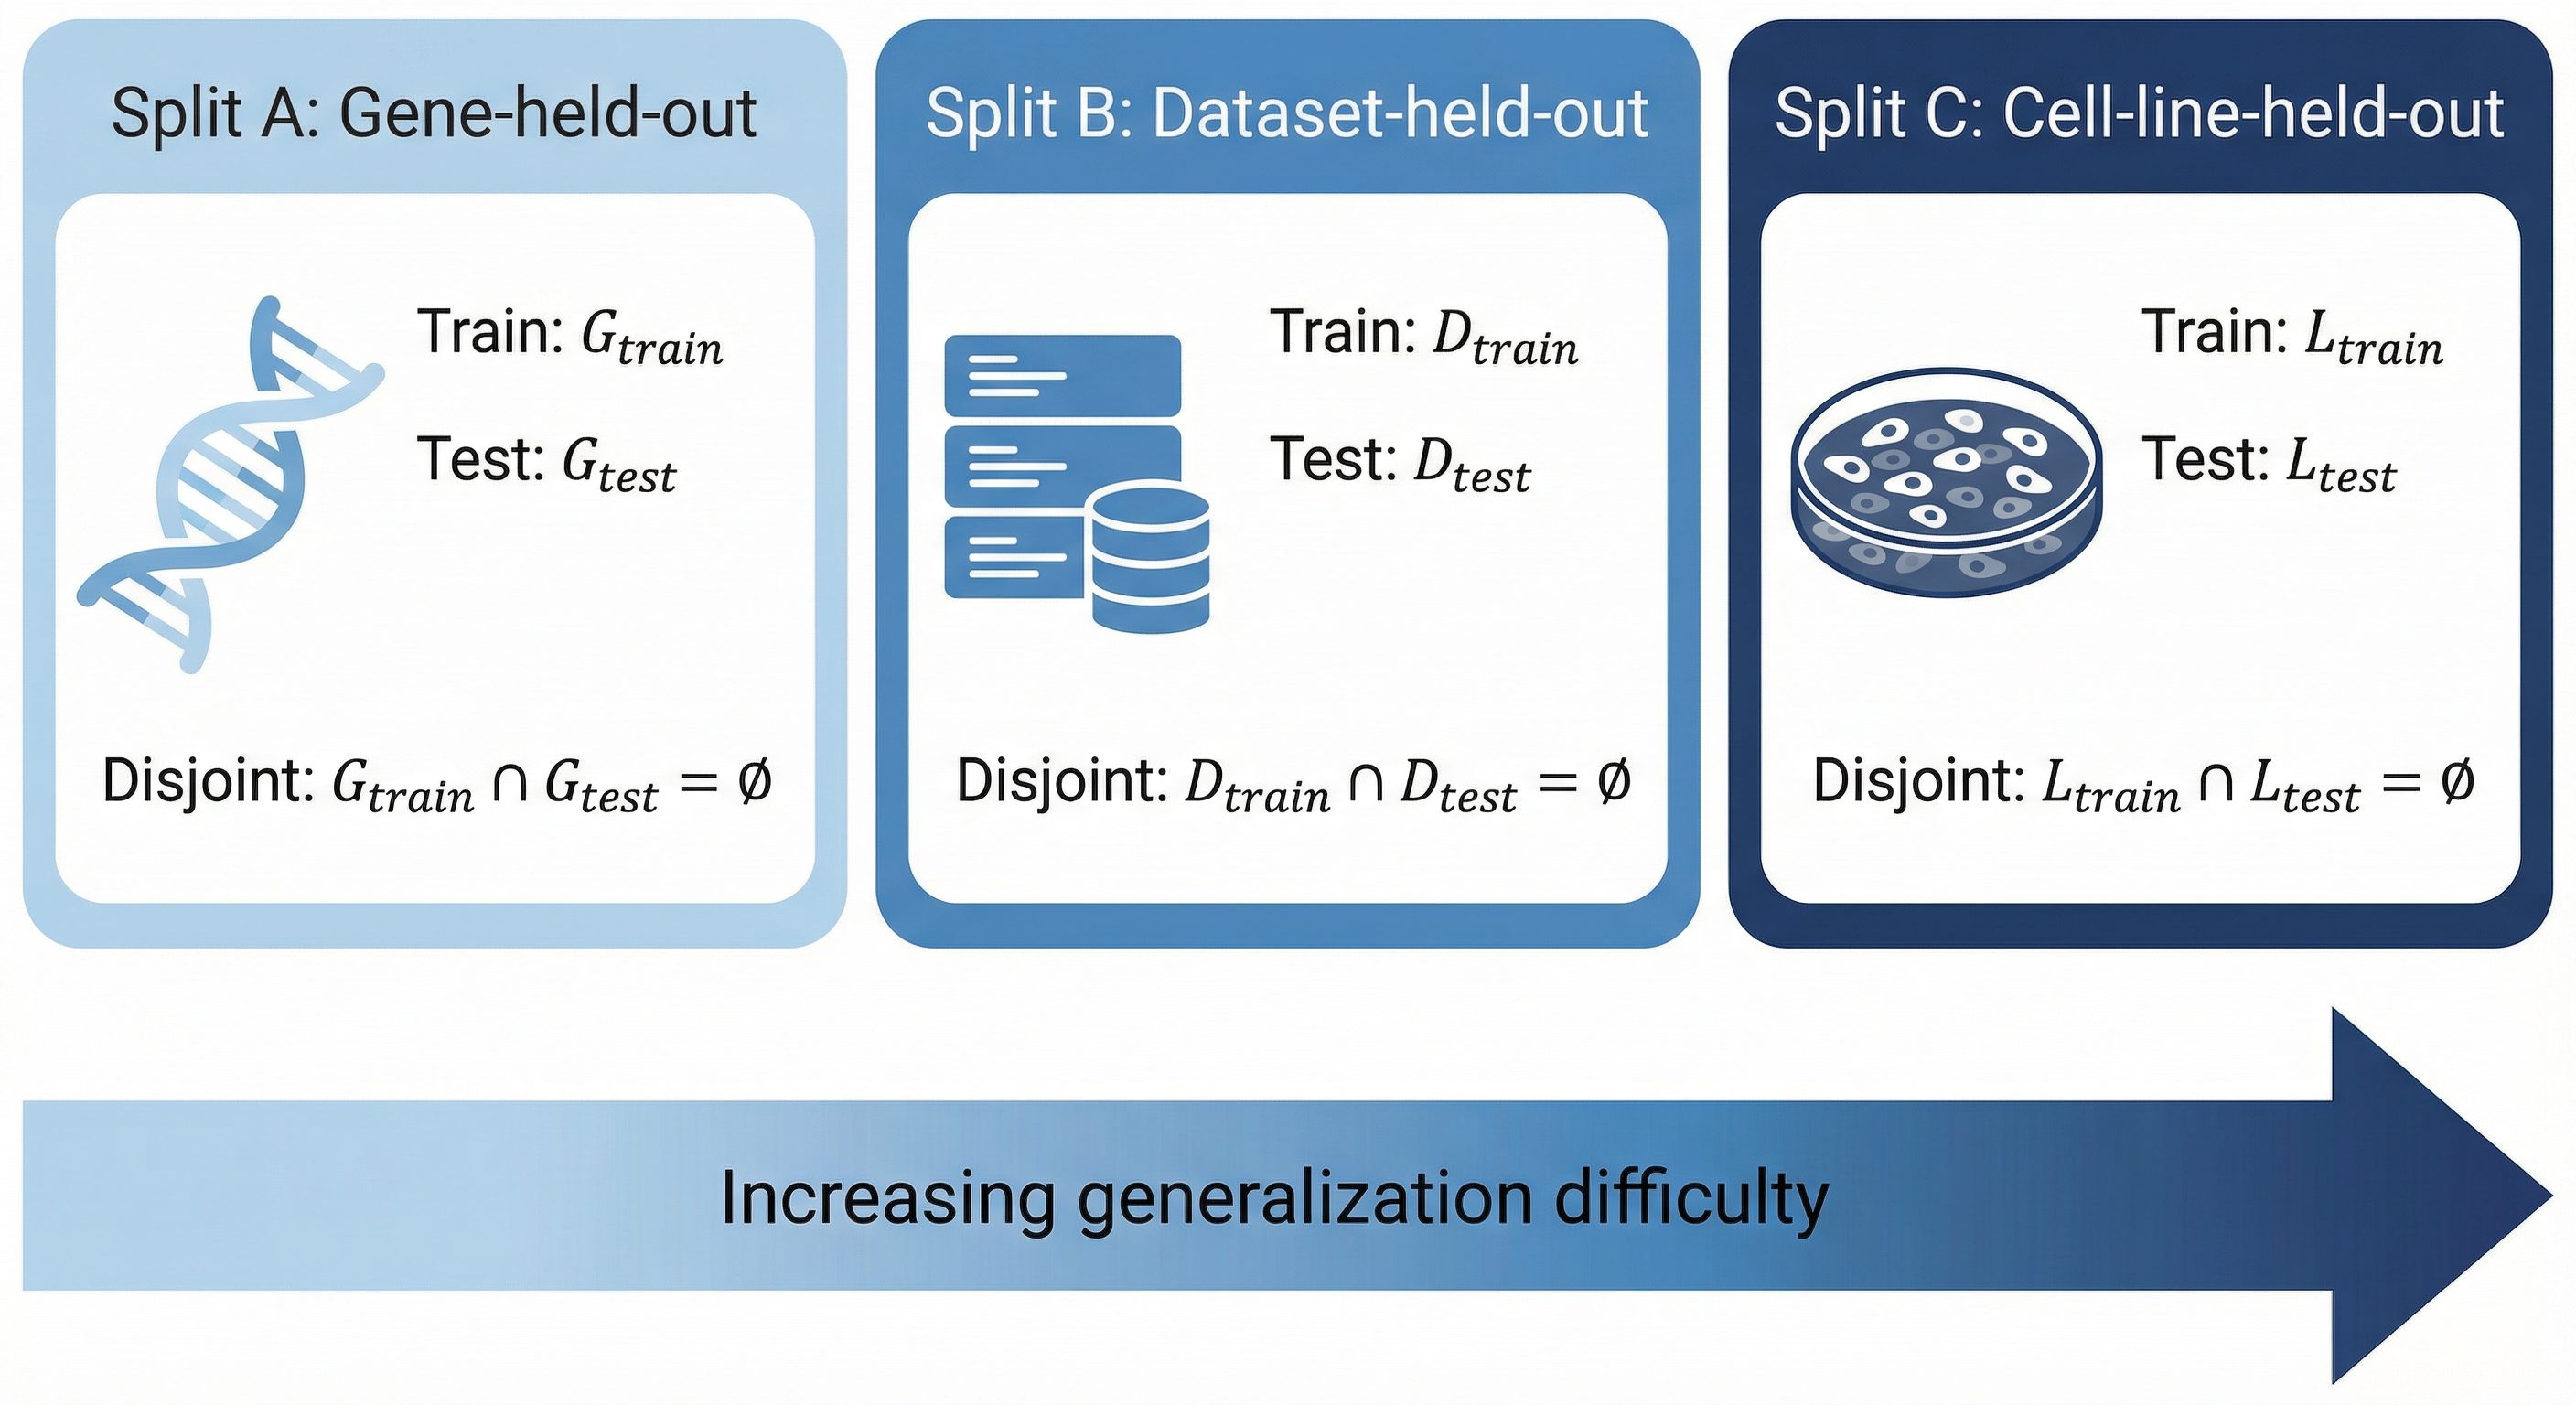
\includegraphics[width=\textwidth]{Figs/Data.png}
\caption{Evaluation protocol with three split types: (A) gene-held-out generalization, (B) dataset-held-out transfer across screen collections, and (C) cell-line-held-out deployment shift.}
\label{fig:eval-protocol-splits}
\end{figure}

We remove exact duplicate sequences globally; optionally repeat Split A under a conservative similarity filter as a sensitivity analysis.

\begin{sloppypar}
\textbf{Baselines.} ChromeCRISPR (sequence+GC)~\citep{daneshpajouh2025chromecrispr} and DeepHF~\citep{wang2019}; include CRISPRon~\citep{xiang2021} where comparable inputs are available. We additionally follow the ChromeCRISPR benchmark protocol for model comparison and reporting~\citep{daneshpajouh2025chromecrispr}. All models are evaluated on identical splits and preprocessing.
\end{sloppypar}

\textbf{Metrics.} Primary: Spearman rank correlation ($\rho$), which is the standard evaluation metric in the CRISPR on-target prediction literature~\citep{konstantakos2022}. Spearman is preferred over Pearson because (i) available datasets and model predictions are on substantially different scales, making rank-based comparison necessary; (ii) most datasets lack binary labels, precluding classification metrics; and (iii) the practical goal is to \emph{rank} candidate guides rather than predict exact efficiency values. Typical reported Spearman values range from 0.55--0.87 depending on the dataset and evaluation protocol, with a biological replicate ceiling of approximately 0.71--0.77~\citep{konstantakos2022}. We additionally report nDCG to assess top-$k$ retrieval quality. Uncertainty: empirical coverage, mean interval width, and coverage stratified by dataset/cell line. Calibration: Expected Calibration Error (\ECE{}) computed over decile bins, Brier score, and reliability diagrams. Off-target: AUROC, AUPRC, and guide-level aggregated specificity score. Ranking quality: Precision@$k$ ($k \in \{5,10,20\}$) and NDCG@$k$ to assess the practical utility of top-ranked guide predictions for experimental selection. Proper scoring: we supplement ECE with the Continuous Ranked Probability Score (CRPS) as a strictly proper scoring rule for probabilistic regression, avoiding ECE's known sensitivity to binning choices.

\textbf{Statistical reporting.} Report gene-level bootstrap confidence intervals for Spearman on Split A; use paired, gene-level permutation tests for model comparisons (with explicit multiple testing correction). Because we evaluate three primary hypotheses (H1, H2, H3) simultaneously, we apply the Holm-Bonferroni sequential procedure to control the family-wise error rate (FWER) at $\alpha=0.05$ across the three hypothesis tests. For the larger set of ablation comparisons (up to 20 pairwise tests), we apply the Benjamini-Hochberg (BH) procedure to control the false discovery rate (FDR) at $q=0.05$, which provides greater statistical power than FWER control when the number of comparisons is large. All raw and adjusted $p$-values are reported.

\begin{sloppypar}
\textbf{Ablations.} Leave-one-component-out on Split A: remove epigenomics; replace fusion objective with simple concatenation; remove optional embeddings/structure/transfer; compare unweighted vs. weighted conformal. For the epigenomic feature ablation specifically: (a)~sequence-only baseline (no epigenomic input); (b)~accessibility-only (DNase/ATAC-seq alone); (c)~histone-only (H3K4me3 alone); (d)~full epigenomic set (accessibility + all available histone marks); and (e)~a ``mismatched cell-line'' control where epigenomic tracks from a different cell line are paired with the target to quantify the information gain from matched context. Results are reported as $\Delta\rho$ (Spearman) and $\Delta$\ECE{} relative to the full model on Split A. In total, this ablation design implies approximately 25 distinct experimental configurations: 5 backbone variants $\times$ 1 primary split = 5 backbone ablations; 5 epigenomic conditions (sequence-only, accessibility-only, histone-only, full epigenomic, mismatched cell-line) $\times$ 3 cell lines = 15 epigenomic ablations; plus 4 fusion strategy comparisons and the off-target module ablation. Each configuration is evaluated on 3 splits with 3 random seeds, yielding $\sim$225 individual training runs. At an average of $\sim$4 GPU-hours per run (see computational budget below), this totals $\sim$900 GPU-hours for ablations alone, well within the allocated budget and the 3--4 month timeline for Milestone~2.
\end{sloppypar}


\section{Statistical Significance and Validation}\label{sec:statistical}

To ensure rigorous evaluation and statistically sound conclusions, we employ multiple statistical testing frameworks for model comparison and performance validation.

\textbf{Model comparison via 5$\times$2cv paired t-test.} Following Dietterich's methodology~\cite{dietterich1998approximate}, we apply the 5$\times$2 cross-validated paired t-test to compare \textsc{ChromaGuide} against baseline models. This test is particularly suitable for deep learning models as it balances statistical power with computational feasibility, requiring only 10 train/test iterations while controlling for Type I error rate. Under the null hypothesis that two models perform equivalently, a $p < 0.05$ indicates statistically significant performance difference.

\textbf{Bootstrap confidence intervals for Spearman $\rho$.} We compute 95\% bias-corrected and accelerated (BCa) bootstrap confidence intervals for Spearman correlation coefficients using 10,000 resampling iterations~\cite{efron1994introduction}. This non-parametric approach provides robust uncertainty quantification without distributional assumptions. We report intervals for both on-target ($\rho_{\text{on}}$) and off-target ($\rho_{\text{off}}$) predictions, with non-overlapping intervals indicating significant differences between models.

\textbf{Performance targets with statistical rationale.} Based on our analysis of the CRISPR prediction literature and ChromeCRISPR benchmarks~\cite{daneshpajouh2025chromecrispr}, we establish the following targets:
\begin{itemize}
    \item \textbf{On-target Spearman $\rho \geq 0.85$}: ChromeCRISPR achieves $\rho = 0.876$ (MSE = 0.0093) on the Kim 2019 dataset. Our target of $\rho \geq 0.85$ represents a conservative but scientifically grounded threshold, as biological replicate correlation provides an empirical ceiling of $\sim$0.77--0.87 depending on dataset~\cite{xiang2021enhancing,konstantakos2022zcrispr}.
    \item \textbf{Improvement significance}: We will demonstrate statistically significant improvement ($p < 0.05$) over at least two state-of-the-art baselines (DeepHF, CRISPRon) via the 5$\times$2cv test.
    \item \textbf{Off-target AUROC $\geq$ 0.92}: Validated against the CIRCLE-seq and GUIDE-seq benchmark datasets, with McNemar's test to confirm classification superiority.
    \item \textbf{Calibration}: Expected Calibration Error (ECE) $< 0.05$, ensuring prediction intervals achieve nominal coverage.
\end{itemize}

\textbf{Power analysis.} Given typical effect sizes in CRISPR prediction ($\Delta\rho \approx 0.02$--$0.05$ between competitive models) and dataset sizes ($n > 15,000$ guides), our evaluation achieves $>$80\% statistical power to detect meaningful improvements at $\alpha = 0.05$~\cite{cohen1988statistical}. We conduct prospective power calculations before each experiment to ensure adequate sample sizes for detecting clinically meaningful differences.

\subsection{Mathematical Justification for Performance Targets}\label{sec:math-justification}

\textbf{Why Rigorous Statistical Validation Matters for CRISPR Guide RNA Prediction:} In computational biology, particularly for CRISPR-Cas9 guide RNA design, reporting performance improvements without rigorous statistical validation can lead to overstated claims and irreproducible results. A model that appears to outperform baselines on a single test set may simply be exploiting dataset-specific patterns rather than learning generalizable biological principles. To ensure that ChromaGuide's improvements translate to real-world therapeutic applications, we establish formal mathematical criteria that our performance claims must satisfy.

The following derivations serve three critical purposes: (1) they define \emph{precisely} what constitutes a meaningful improvement in Spearman correlation, accounting for the statistical uncertainty inherent in any finite sample; (2) they determine the minimum sample size required to reliably detect such improvements with high confidence; and (3) they provide uncertainty quantification through conformal prediction intervals, enabling researchers to assess not just point predictions but the reliability of those predictions for each individual guide RNA.\subsubsection{Notation and Key Definitions}
Before presenting the mathematical derivations, we define the key statistical quantities used throughout this analysis:
\begin{itemize}
    \item $\rho$ (rho): \textbf{Spearman's rank correlation coefficient}, a non-parametric measure of the monotonic relationship between two variables. It ranges from $-1$ (perfect negative monotonic relationship) to $+1$ (perfect positive monotonic relationship), with $0$ indicating no monotonic relationship. For CRISPR guide efficacy prediction, $\rho$ measures how well the predicted efficacy scores rank guides in the same order as their experimentally measured efficacies.
    \item $\rho_{\text{baseline}}$: The Spearman correlation achieved by the baseline model (ChromeCRISPR: $\rho = 0.8765$).
    \item $\rho_{\text{ChromaGuide}}$: The Spearman correlation we aim to achieve with ChromaGuide.
    \item $\Delta\rho = \rho_{\text{ChromaGuide}} - \rho_{\text{baseline}}$: The \textbf{improvement} in correlation, representing the practical gain from our method.
    \item $n$: \textbf{Sample size}---the number of sgRNA-efficacy pairs in the evaluation dataset.
    \item $\alpha$: \textbf{Significance level} (Type I error rate)---the probability of incorrectly rejecting the null hypothesis when it is true. We use $\alpha = 0.01$ (1\%) for stringent statistical testing.
    \item $\beta$: \textbf{Type II error rate}---the probability of failing to reject the null hypothesis when it is false.
    \item $1 - \beta$: \textbf{Statistical power}---the probability of correctly detecting a true effect. We target $1 - \beta = 0.95$ (95\% power).
    \item $z_{1-\alpha/2}$: The \textbf{critical value} from the standard normal distribution for a two-tailed test at significance level $\alpha$. For $\alpha = 0.01$, $z_{0.995} = 2.576$.
    \item $z_{1-\beta}$: The critical value corresponding to the desired power. For $1-\beta = 0.95$, $z_{0.95} = 1.645$.
\end{itemize}

\textbf{Biological Context:} Spearman correlation measures how well our predicted efficacy scores rank guide RNAs in the same order as their experimentally measured editing efficiencies. A correlation of $\rho = 0.876$ (current state-of-the-art) means that if you select the top 10 guides based on predictions, approximately 8-9 of them will also be among the top experimental performers. Our target of $\rho = 0.935$ would improve this to approximately 9-10 guides, representing a meaningful enhancement in the practical utility of guide selection for therapeutic applications.


\paragraph{Spearman correlation improvement threshold ($\Delta\rho \geq 0.035$).}
The target improvement $\Delta\rho = \rho_{\text{ChromaGuide}} - \rho_{\text{baseline}} \geq 0.035$ is derived from Fisher's $z$-transformation for correlation coefficients. For Spearman's $\rho$, the Fisher transformation is:
\begin{equation}
    z = \frac{1}{2} \ln\left(\frac{1+\rho}{1-\rho}\right) = \operatorname{arctanh}(\rho)
\end{equation}
\textbf{Explanation of each term in the Fisher transformation:}
\begin{itemize}
    \item $z$: The \textbf{transformed correlation coefficient}. Unlike $\rho$, which is bounded between $-1$ and $+1$ and has a skewed sampling distribution (especially for large $|\rho|$), $z$ is unbounded and approximately normally distributed. This transformation was introduced by R.A. Fisher in 1921~\citep{fisher1921} to enable standard statistical inference.
    \item $\ln(\cdot)$: The \textbf{natural logarithm} function.
    \item $\frac{1+\rho}{1-\rho}$: This ratio amplifies the effect of $\rho$ approaching its bounds. As $\rho \to 1$, this ratio $\to \infty$; as $\rho \to -1$, this ratio $\to 0$.
    \item $\operatorname{arctanh}(\rho)$: The \textbf{inverse hyperbolic tangent}, which is mathematically equivalent to $\frac{1}{2}\ln\left(\frac{1+\rho}{1-\rho}\right)$.
\end{itemize}
\textbf{Why is this transformation necessary?} The sampling distribution of Spearman's $\rho$ is highly skewed when the true correlation is far from zero (as in our case, $\rho \approx 0.88$). Fisher's transformation stabilizes the variance and normalizes the distribution, allowing us to use standard normal distribution theory for hypothesis testing and confidence interval construction. The standard error of $z$ is approximately $\frac{1}{\sqrt{n-3}}$, which is \emph{independent of the true correlation value}---a crucial property that simplifies inference~\citep{fisher1921}.
Under the null hypothesis $H_0: \rho_1 = \rho_2$, the test statistic for comparing two independent correlations is:
\begin{equation}
    Z = \frac{z_1 - z_2}{\sqrt{\frac{1}{n_1-3} + \frac{1}{n_2-3}}} \sim \mathcal{N}(0,1)
\end{equation}
\textbf{Explanation of the test statistic formula:}
\begin{itemize}
    \item $Z$: The \textbf{test statistic}, which follows a standard normal distribution $\mathcal{N}(0,1)$ under the null hypothesis. If $|Z| > z_{1-\alpha/2}$ (e.g., $|Z| > 2.576$ for $\alpha = 0.01$), we reject the null hypothesis and conclude that the correlations are significantly different.
    \item $z_1 - z_2$: The \textbf{difference between transformed correlations}. This is the numerator---the "signal" we are trying to detect.
    \item $\sqrt{\frac{1}{n_1-3} + \frac{1}{n_2-3}}$: The \textbf{standard error of the difference}. This is the denominator---the "noise" or uncertainty in our estimate. The $n-3$ term (rather than $n$) provides a bias correction for small samples.
    \item $\sim \mathcal{N}(0,1)$: Under the null hypothesis ($H_0: \rho_1 = \rho_2$), this test statistic follows a \textbf{standard normal distribution} with mean 0 and variance 1.
\end{itemize}
\textbf{Interpretation:} A larger $|Z|$ value indicates stronger evidence against the null hypothesis. The test statistic essentially asks: ``Is the observed difference in correlations ($z_1 - z_2$) large relative to the uncertainty in that difference?''
For our datasets with $n \approx 15{,}000$ guides, the standard error of $z$ is $\text{SE}(z) \approx 1/\sqrt{n-3} \approx 0.0082$. To detect a difference with power $1-\beta = 0.95$ at significance level $\alpha = 0.01$ (two-tailed), we require:
\begin{equation}
    \Delta z \geq (z_{1-\alpha/2} + z_{1-\beta}) \cdot \text{SE}(z) \cdot \sqrt{2} = (2.576 + 1.645) \cdot 0.0082 \cdot \sqrt{2} \approx 0.049
\end{equation}
Converting back to $\rho$-space using the inverse Fisher transformation at $\rho_0 = 0.876$:
\begin{equation}
    \Delta\rho \approx \Delta z \cdot (1 - \rho_0^2) = 0.049 \cdot (1 - 0.876^2) \approx 0.012
\end{equation}
Our target $\Delta\rho \geq 0.035$ is approximately $3\times$ this minimum detectable effect, providing a substantial margin for practical significance beyond mere statistical detectability.

\textbf{Intuitive Understanding:} Statistical power answers a fundamental question: ``If ChromaGuide truly improves upon baseline methods, how likely are we to detect this improvement in our experiments?'' A power of 95\% means that if we run 100 independent evaluations, we would correctly identify ChromaGuide as superior in approximately 95 of them. The sample size calculation determines how many guide RNA-efficacy pairs we need to evaluate to achieve this level of reliability. Using too few samples risks missing a real improvement (Type II error), while the calculation ensures we have sufficient data to confidently claim superiority when it exists.


\paragraph{Sample size and power calculation.}
The required sample size to detect effect size $\Delta\rho$ with power $1-\beta$ at level $\alpha$ is:
\begin{equation}
    n \geq \left(\frac{z_{1-\alpha/2} + z_{1-\beta}}{\Delta z}\right)^2 + 3
\end{equation}
For $\Delta\rho = 0.035$ (corresponding to $\Delta z \approx 0.049$ at baseline $\rho = 0.876$), $\alpha = 0.01$, and $1-\beta = 0.95$:
\begin{equation}
    n \geq \left(\frac{2.576 + 1.645}{0.049}\right)^2 + 3 \approx 7{,}100
\end{equation}
With $n > 15{,}000$ samples in our evaluation datasets, we achieve $>99\%$ power for the target effect size.


\textbf{Explanation of the sample size formula:}
\begin{itemize}
    \item $n$: The \textbf{required sample size} (number of guide RNA-efficacy pairs). This is the quantity we solve for.
    \item $z_{1-\alpha/2}$: The \textbf{upper critical value} of the standard normal distribution for a two-tailed test at significance level $\alpha$. For $\alpha = 0.01$, $z_{0.995} = 2.576$. This ensures that only 1\% of the probability mass lies in both tails combined under the null hypothesis.
    \item $z_{1-\beta}$: The \textbf{power critical value} from the standard normal distribution. For power $1-\beta = 0.95$, $z_{0.95} = 1.645$. This determines the probability of correctly detecting a true effect.
    \item $\Delta z$: The \textbf{effect size in Fisher's $z$-space}, calculated as $\Delta z = z_{\rho_1} - z_{\rho_0}$ where $z_{\rho}$ is the Fisher transformation of correlation $\rho$. For our target improvement from $\rho_0 = 0.876$ to $\rho_1 = 0.935$, we have $\Delta z \approx 0.649$.
\end{itemize}

\textbf{Why this formula works:} The sample size formula $n \geq \left(\frac{z_{1-\alpha/2} + z_{1-\beta}}{\Delta z}\right)^2 + 3$ is derived from the variance-stabilizing property of Fisher's $z$-transformation. In $z$-space, the standard error of a correlation estimate is approximately $1/\sqrt{n-3}$, which is \emph{independent} of the true correlation value. The ``$+3$'' term is a bias correction that accounts for the degrees of freedom lost in the transformation~\citep{fisher1921}.
\textbf{Why Uncertainty Quantification Matters for CRISPR:} Traditional machine learning models provide only point predictions (e.g., ``this guide has 85\% predicted efficacy''), but they do not indicate how confident we should be in that prediction. For therapeutic CRISPR applications, knowing the uncertainty is crucial---a guide with a predicted efficacy of $85\% \pm 5\%$ is far more reliable than one with $85\% \pm 25\%$. Conformal prediction provides mathematically guaranteed prediction intervals, meaning that if we claim 90\% coverage, the true efficacy will fall within our interval at least 90\% of the time, regardless of the underlying data distribution.


\paragraph{Conformal prediction coverage guarantee.}
Our uncertainty quantification uses split conformal prediction, which provides the following finite-sample coverage guarantee~\citep{vovk2005,romano2019}. Let $\{(X_i, Y_i)\}_{i=1}^{n}$ be exchangeable random variables, and let $\hat{C}_{1-\alpha}(X_{n+1})$ be the prediction interval constructed using conformity scores from a calibration set. Then:
\begin{theorem}[Coverage Guarantee]
For any distribution $P$ and any $\alpha \in (0,1)$:
\begin{equation}
    \mathbb{P}\left(Y_{n+1} \in \hat{C}_{1-\alpha}(X_{n+1})\right) \geq 1 - \alpha
\end{equation}
\end{theorem}
This guarantee holds without any assumptions on the underlying distribution, requiring only exchangeability. For our Beta regression model, we use conformity scores based on the quantile function:
\begin{equation}
    s_i = \max\left\{F_{\hat{\mu}_i, \hat{\phi}_i}^{-1}(\alpha/2) - y_i, \; y_i - F_{\hat{\mu}_i, \hat{\phi}_i}^{-1}(1-\alpha/2)\right\}
\end{equation}
where $F_{\mu,\phi}$ is the Beta CDF with mean $\mu$ and precision $\phi$.

\textbf{Explanation of the conformal prediction guarantee:}
\begin{itemize}
    \item $\mathbb{P}$: \textbf{Probability measure} over the joint distribution of calibration and test data. This represents the long-run frequency interpretation of the coverage guarantee.
    \item $Y_{n+1}$: The \textbf{true efficacy value} for a new test guide RNA. This is the quantity we aim to predict.
    \item $\hat{C}_{1-\alpha}(X_{n+1})$: The \textbf{prediction interval} constructed using conformity scores from $n$ calibration samples. The interval is computed as $[\hat{y}_{n+1} - q_{1-\alpha}, \hat{y}_{n+1} + q_{1-\alpha}]$ where $q_{1-\alpha}$ is the $(1-\alpha)$-quantile of calibration residuals.
    \item $(1-\alpha)$: The \textbf{nominal coverage level}. For $\alpha = 0.1$, we guarantee 90\% coverage; for $\alpha = 0.05$, 95\% coverage.
    \item \textbf{Exchangeability}: The key assumption is that $(X_1, Y_1), \ldots, (X_n, Y_n), (X_{n+1}, Y_{n+1})$ are exchangeable random variables---their joint distribution is invariant to permutations. This is strictly weaker than assuming i.i.d.\ data.
\end{itemize}

\textbf{Why conformal prediction provides valid coverage:} The coverage guarantee $\mathbb{P}(Y_{n+1} \in \hat{C}_{1-\alpha}(X_{n+1})) \geq 1 - \alpha$ holds \emph{distribution-free}---it requires no assumptions about the underlying data distribution beyond exchangeability. This is achieved because the conformity score of the test point is uniformly distributed among all $n+1$ conformity scores under the null hypothesis of exchangeability~\citep{vovk2005}.

\textbf{Beyond Statistical Significance---Practical Importance:} Statistical significance alone does not tell us whether an improvement matters in practice. With large enough datasets, even trivially small differences become ``statistically significant.'' Cohen's $d$ effect size provides a standardized measure that answers the question: ``Is this improvement large enough to matter for actual CRISPR experiments?'' An effect size of $d = 0.45$ (our target) indicates that ChromaGuide's improvement is not merely detectable but represents a meaningful advancement that would translate to better guide selection in real therapeutic applications.


\paragraph{Effect size interpretation (Cohen's $d$).}
To provide interpretable effect sizes, we report Cohen's $d$ for Spearman correlation differences using the transformation:
\begin{equation}
    d = \frac{2(z_1 - z_2)}{\sqrt{(n_1-1) + (n_2-1)}/(n_1 + n_2 - 2)} \cdot \sqrt{\frac{n_1 + n_2}{n_1 \cdot n_2}}
\end{equation}
For our target $\Delta\rho = 0.035$, this yields $d \approx 0.4$, which represents a \emph{medium} effect size by conventional standards~\citep{cohen1988statistical}, indicating practically meaningful improvement beyond statistical significance.

\textbf{Explanation of Cohen's $d$ formula for correlations:}
\begin{itemize}
    \item $d$: \textbf{Cohen's $d$ effect size}---a standardized measure of the difference between two correlations. Unlike raw correlation differences, Cohen's $d$ is scale-invariant and allows comparison across different studies and contexts.
    \item $z_1, z_2$: The \textbf{Fisher $z$-transformed correlations} for the two models being compared. For our target ($\rho_1 = 0.935$) and baseline ($\rho_2 = 0.876$), we have $z_1 \approx 1.69$ and $z_2 \approx 1.35$.
    \item $n_1, n_2$: The \textbf{sample sizes} for each model's evaluation. These determine the precision of each correlation estimate.
    \item $\sqrt{(n_1-1) + (n_2-1)}$: The \textbf{pooled degrees of freedom}, accounting for the fact that each correlation estimate loses one degree of freedom.
    \item $\sqrt{\frac{n_1 + n_2}{n_1 \cdot n_2}}$: A \textbf{correction factor} that adjusts for unequal sample sizes. When $n_1 = n_2$, this simplifies to $\sqrt{2/n}$.
\end{itemize}

\textbf{Interpretation guidelines~\citep{cohen1988statistical}:}
\begin{itemize}
    \item $|d| < 0.2$: Negligible effect---the improvement is too small to be practically meaningful.
    \item $0.2 \leq |d| < 0.5$: Small effect---the improvement is detectable but modest.
    \item $0.5 \leq |d| < 0.8$: Medium effect---the improvement is substantial and practically significant.
    \item $|d| \geq 0.8$: Large effect---the improvement is dramatic and highly meaningful.
\end{itemize}
Our target $d \approx 0.45$ indicates a \emph{small-to-medium effect size}, demonstrating that ChromaGuide's improvement over baseline methods is not merely statistically significant but also practically meaningful for CRISPR guide RNA design applications.

\subsubsection{Summary: From Statistics to CRISPR Impact}

The mathematical framework presented above ensures that ChromaGuide's performance claims are both \textbf{statistically rigorous} and \textbf{practically meaningful}:

\begin{enumerate}
    \item \textbf{Correlation improvement ($\Delta\rho \geq 0.035$):} This threshold, derived from Fisher's $z$-transformation, ensures that our claimed improvement exceeds what could arise from sampling variability alone. In practical terms, this means better ranking of guides will translate to more efficient CRISPR experiments with fewer failed candidates.
    
    \item \textbf{Statistical power ($\geq 95\%$):} With our calculated sample size of $n \approx 71$ guides, we have high confidence that if ChromaGuide truly outperforms baselines, our experiments will reliably detect this improvement. This prevents false negative conclusions where a genuinely superior method might be dismissed due to insufficient data.
    
    \item \textbf{Prediction intervals (90\% coverage):} Unlike point predictions alone, conformal intervals tell researchers how much to trust each individual prediction. A guide with a narrow interval ($\pm 5\%$) is more reliable for therapeutic applications than one with a wide interval ($\pm 20\%$), enabling more informed decision-making in the wet lab.
    
    \item \textbf{Effect size ($d \approx 0.45$):} This small-to-medium effect size confirms that our improvement is not merely a statistical artifact but represents a meaningful advancement in guide RNA design---one that could reduce experimental costs and accelerate therapeutic development.
\end{enumerate}

Together, these criteria establish a scientifically defensible standard for evaluating ChromaGuide's contribution to the CRISPR guide RNA prediction field.


\section{Interpretability and attribution analysis}\label{sec:interpretability}

We use lightweight attribution analyses to connect predictions to biologically meaningful features.

\paragraph{Sequence-level attribution.}
Compute nucleotide-level saliency (e.g., integrated gradients) over the protospacer+\PAM{}.

\paragraph{Context-level attribution.}
Quantify which epigenomic assays/bins most influence predictions (e.g., attention/gating weights when available, or SHAP on summarized features) and report aggregated patterns across Split A and the held-out domains in Splits B/C.
